% Options for packages loaded elsewhere
\PassOptionsToPackage{unicode}{hyperref}
\PassOptionsToPackage{hyphens}{url}
\PassOptionsToPackage{dvipsnames,svgnames,x11names}{xcolor}
%
\documentclass[
  letterpaper,
  DIV=11,
  numbers=noendperiod]{scrartcl}

\usepackage{amsmath,amssymb}
\usepackage{iftex}
\ifPDFTeX
  \usepackage[T1]{fontenc}
  \usepackage[utf8]{inputenc}
  \usepackage{textcomp} % provide euro and other symbols
\else % if luatex or xetex
  \usepackage{unicode-math}
  \defaultfontfeatures{Scale=MatchLowercase}
  \defaultfontfeatures[\rmfamily]{Ligatures=TeX,Scale=1}
\fi
\usepackage{lmodern}
\ifPDFTeX\else  
    % xetex/luatex font selection
\fi
% Use upquote if available, for straight quotes in verbatim environments
\IfFileExists{upquote.sty}{\usepackage{upquote}}{}
\IfFileExists{microtype.sty}{% use microtype if available
  \usepackage[]{microtype}
  \UseMicrotypeSet[protrusion]{basicmath} % disable protrusion for tt fonts
}{}
\makeatletter
\@ifundefined{KOMAClassName}{% if non-KOMA class
  \IfFileExists{parskip.sty}{%
    \usepackage{parskip}
  }{% else
    \setlength{\parindent}{0pt}
    \setlength{\parskip}{6pt plus 2pt minus 1pt}}
}{% if KOMA class
  \KOMAoptions{parskip=half}}
\makeatother
\usepackage{xcolor}
\setlength{\emergencystretch}{3em} % prevent overfull lines
\setcounter{secnumdepth}{-\maxdimen} % remove section numbering
% Make \paragraph and \subparagraph free-standing
\ifx\paragraph\undefined\else
  \let\oldparagraph\paragraph
  \renewcommand{\paragraph}[1]{\oldparagraph{#1}\mbox{}}
\fi
\ifx\subparagraph\undefined\else
  \let\oldsubparagraph\subparagraph
  \renewcommand{\subparagraph}[1]{\oldsubparagraph{#1}\mbox{}}
\fi

\usepackage{color}
\usepackage{fancyvrb}
\newcommand{\VerbBar}{|}
\newcommand{\VERB}{\Verb[commandchars=\\\{\}]}
\DefineVerbatimEnvironment{Highlighting}{Verbatim}{commandchars=\\\{\}}
% Add ',fontsize=\small' for more characters per line
\usepackage{framed}
\definecolor{shadecolor}{RGB}{241,243,245}
\newenvironment{Shaded}{\begin{snugshade}}{\end{snugshade}}
\newcommand{\AlertTok}[1]{\textcolor[rgb]{0.68,0.00,0.00}{#1}}
\newcommand{\AnnotationTok}[1]{\textcolor[rgb]{0.37,0.37,0.37}{#1}}
\newcommand{\AttributeTok}[1]{\textcolor[rgb]{0.40,0.45,0.13}{#1}}
\newcommand{\BaseNTok}[1]{\textcolor[rgb]{0.68,0.00,0.00}{#1}}
\newcommand{\BuiltInTok}[1]{\textcolor[rgb]{0.00,0.23,0.31}{#1}}
\newcommand{\CharTok}[1]{\textcolor[rgb]{0.13,0.47,0.30}{#1}}
\newcommand{\CommentTok}[1]{\textcolor[rgb]{0.37,0.37,0.37}{#1}}
\newcommand{\CommentVarTok}[1]{\textcolor[rgb]{0.37,0.37,0.37}{\textit{#1}}}
\newcommand{\ConstantTok}[1]{\textcolor[rgb]{0.56,0.35,0.01}{#1}}
\newcommand{\ControlFlowTok}[1]{\textcolor[rgb]{0.00,0.23,0.31}{#1}}
\newcommand{\DataTypeTok}[1]{\textcolor[rgb]{0.68,0.00,0.00}{#1}}
\newcommand{\DecValTok}[1]{\textcolor[rgb]{0.68,0.00,0.00}{#1}}
\newcommand{\DocumentationTok}[1]{\textcolor[rgb]{0.37,0.37,0.37}{\textit{#1}}}
\newcommand{\ErrorTok}[1]{\textcolor[rgb]{0.68,0.00,0.00}{#1}}
\newcommand{\ExtensionTok}[1]{\textcolor[rgb]{0.00,0.23,0.31}{#1}}
\newcommand{\FloatTok}[1]{\textcolor[rgb]{0.68,0.00,0.00}{#1}}
\newcommand{\FunctionTok}[1]{\textcolor[rgb]{0.28,0.35,0.67}{#1}}
\newcommand{\ImportTok}[1]{\textcolor[rgb]{0.00,0.46,0.62}{#1}}
\newcommand{\InformationTok}[1]{\textcolor[rgb]{0.37,0.37,0.37}{#1}}
\newcommand{\KeywordTok}[1]{\textcolor[rgb]{0.00,0.23,0.31}{#1}}
\newcommand{\NormalTok}[1]{\textcolor[rgb]{0.00,0.23,0.31}{#1}}
\newcommand{\OperatorTok}[1]{\textcolor[rgb]{0.37,0.37,0.37}{#1}}
\newcommand{\OtherTok}[1]{\textcolor[rgb]{0.00,0.23,0.31}{#1}}
\newcommand{\PreprocessorTok}[1]{\textcolor[rgb]{0.68,0.00,0.00}{#1}}
\newcommand{\RegionMarkerTok}[1]{\textcolor[rgb]{0.00,0.23,0.31}{#1}}
\newcommand{\SpecialCharTok}[1]{\textcolor[rgb]{0.37,0.37,0.37}{#1}}
\newcommand{\SpecialStringTok}[1]{\textcolor[rgb]{0.13,0.47,0.30}{#1}}
\newcommand{\StringTok}[1]{\textcolor[rgb]{0.13,0.47,0.30}{#1}}
\newcommand{\VariableTok}[1]{\textcolor[rgb]{0.07,0.07,0.07}{#1}}
\newcommand{\VerbatimStringTok}[1]{\textcolor[rgb]{0.13,0.47,0.30}{#1}}
\newcommand{\WarningTok}[1]{\textcolor[rgb]{0.37,0.37,0.37}{\textit{#1}}}

\providecommand{\tightlist}{%
  \setlength{\itemsep}{0pt}\setlength{\parskip}{0pt}}\usepackage{longtable,booktabs,array}
\usepackage{calc} % for calculating minipage widths
% Correct order of tables after \paragraph or \subparagraph
\usepackage{etoolbox}
\makeatletter
\patchcmd\longtable{\par}{\if@noskipsec\mbox{}\fi\par}{}{}
\makeatother
% Allow footnotes in longtable head/foot
\IfFileExists{footnotehyper.sty}{\usepackage{footnotehyper}}{\usepackage{footnote}}
\makesavenoteenv{longtable}
\usepackage{graphicx}
\makeatletter
\def\maxwidth{\ifdim\Gin@nat@width>\linewidth\linewidth\else\Gin@nat@width\fi}
\def\maxheight{\ifdim\Gin@nat@height>\textheight\textheight\else\Gin@nat@height\fi}
\makeatother
% Scale images if necessary, so that they will not overflow the page
% margins by default, and it is still possible to overwrite the defaults
% using explicit options in \includegraphics[width, height, ...]{}
\setkeys{Gin}{width=\maxwidth,height=\maxheight,keepaspectratio}
% Set default figure placement to htbp
\makeatletter
\def\fps@figure{htbp}
\makeatother

\KOMAoption{captions}{tablesignature}
\makeatletter
\@ifpackageloaded{caption}{}{\usepackage{caption}}
\AtBeginDocument{%
\ifdefined\contentsname
  \renewcommand*\contentsname{Table of contents}
\else
  \newcommand\contentsname{Table of contents}
\fi
\ifdefined\listfigurename
  \renewcommand*\listfigurename{List of Figures}
\else
  \newcommand\listfigurename{List of Figures}
\fi
\ifdefined\listtablename
  \renewcommand*\listtablename{List of Tables}
\else
  \newcommand\listtablename{List of Tables}
\fi
\ifdefined\figurename
  \renewcommand*\figurename{Figure}
\else
  \newcommand\figurename{Figure}
\fi
\ifdefined\tablename
  \renewcommand*\tablename{Table}
\else
  \newcommand\tablename{Table}
\fi
}
\@ifpackageloaded{float}{}{\usepackage{float}}
\floatstyle{ruled}
\@ifundefined{c@chapter}{\newfloat{codelisting}{h}{lop}}{\newfloat{codelisting}{h}{lop}[chapter]}
\floatname{codelisting}{Listing}
\newcommand*\listoflistings{\listof{codelisting}{List of Listings}}
\makeatother
\makeatletter
\makeatother
\makeatletter
\@ifpackageloaded{caption}{}{\usepackage{caption}}
\@ifpackageloaded{subcaption}{}{\usepackage{subcaption}}
\makeatother
\ifLuaTeX
  \usepackage{selnolig}  % disable illegal ligatures
\fi
\usepackage{bookmark}

\IfFileExists{xurl.sty}{\usepackage{xurl}}{} % add URL line breaks if available
\urlstyle{same} % disable monospaced font for URLs
\hypersetup{
  pdftitle={Pooled swab sampling for pathogen early detection},
  pdfauthor={Simon Grimm},
  colorlinks=true,
  linkcolor={blue},
  filecolor={Maroon},
  citecolor={Blue},
  urlcolor={Blue},
  pdfcreator={LaTeX via pandoc}}

\title{Pooled swab sampling for pathogen early detection}
\author{Simon Grimm}
\date{2024-02-23}

\begin{document}
\maketitle

\begin{Shaded}
\begin{Highlighting}[]
\CommentTok{\# Importing packages}
\ImportTok{import}\NormalTok{ seaborn }\ImportTok{as}\NormalTok{ sns}
\ImportTok{import}\NormalTok{ pandas }\ImportTok{as}\NormalTok{ pd}
\ImportTok{import}\NormalTok{ matplotlib.pyplot }\ImportTok{as}\NormalTok{ plt}
\ImportTok{import}\NormalTok{ numpy }\ImportTok{as}\NormalTok{ np}
\ImportTok{from}\NormalTok{ collections }\ImportTok{import}\NormalTok{ defaultdict}
\ImportTok{import}\NormalTok{ random}
\ImportTok{import}\NormalTok{ math}
\end{Highlighting}
\end{Shaded}

\section{Introduction}\label{introduction}

The NAO aims to detect stealth pathogens at an early stage. Up until, we
have have focused much our research on wastewater treatment plant (WTP)
samples. While WTP sampling offers some advantages, its limitations
include environmental noise, non-human biological material, and low
pathogen abundance. The NAO thus also wants to investigate other
sampling approaches. To this end we've previously researched the promise
of air sampling for pathogen early detection, and Will recently created
a framework that allows analysis of various types of sampling
strategies.

One promising approach is sampling using nasal, nasopharyngeal (NP), or
oropharyngeal (OP) swabs. When pooled, these samples have several
advantages

\begin{itemize}
\tightlist
\item
  400x higher RA(1\%) than wastewater, atleast based on an initial
  BOTEC, that I have low confidence in.
\item
  More metadata on individuals that contributed to the sample (because
  you can have them provide some basic metadata when providing the
  sample.
\item
  Potentially less static complexity than wastewater.
\item
  If pools are large enough, dynamic complexity could also be lower.
\item
  There is more existing research on swab sampling than on other sample
  types.
\end{itemize}

Still, the approach also has downsides:

\begin{itemize}
\tightlist
\item
  If not sampling at an airport, getting wide geographic coverage is
  harder.
\item
  Scaling is more expensive than with wastewater, especially increasing
  the number of samples provided at at given location.
\item
  Regulatory hurdles are likely higher than when sampling wastewater.
\end{itemize}

\section{Pathogen abundance and detection
capability}\label{pathogen-abundance-and-detection-capability}

\subsection{Pathogen shedding}\label{pathogen-shedding}

Among many types of pathogens, respiratory pathogens are particularly
likely to cause future pandemics (Amesh A. Adalja, MD, Matthew Watson,
\ldots). Though different pathogens have different tropism across
tissues (SARS-CoV-2 having a wider wider tropism than influenza
(Flerlage et al.~2021)), all of them are respiratory pathogens and thus
shed in the respiratory tract, which includes the pharynx, mouth, and
nose.

In a swab sampling program we could use different swabs that target any
of these sitesm, i.e., the nostrils, the nasopharynx, oropharynx, and
the mid-turbinate region\footnote{The mid-turbinate region is the area
  between the nasal opening (Nares) and the nasopharynx.}. These sites
differ in their comfort of sampling and (probably) in their sensitivity.
For instance, nasopharyngeal swabs (NP swabs) would have be far better
than other swabs for us to consider them for a sampling program, given
that they do not allow self-sampling.

We will evaluate the performance of different swab types in three ways:

\begin{itemize}
\tightlist
\item
  \textbf{Sensitivity}: Is the pathogen present at all?
\item
  \textbf{Viral load}: How much of the pathogen can be measured? This
  metric is based on the qPCR cycle threshold of quantiative.
\item
  \textbf{Relative abundance}: When performing untargeted sequencing,
  what is the relative abundance of a pathogen?
\end{itemize}

\subsubsection{Sensitivity of different swab
types}\label{sensitivity-of-different-swab-types}

(Tsang et al.~2021) performed a meta-analysis to evaluate the ability of
different swab types in detecting SARS-CoV-2 using qPCR. Swab types
included nasal swabs (n=1622), throat swabs (n=388), and pooled nasal
and throat swabs (n=719), each of which were compared to nasopharyngeal
swabs. Overall, pooled nasal/throat swabs have the best diagnostic
performance with sensitivity of 0.97 (0.93-1.00).

\begin{longtable}[]{@{}
  >{\raggedright\arraybackslash}p{(\columnwidth - 8\tabcolsep) * \real{0.2586}}
  >{\raggedright\arraybackslash}p{(\columnwidth - 8\tabcolsep) * \real{0.1379}}
  >{\raggedright\arraybackslash}p{(\columnwidth - 8\tabcolsep) * \real{0.1379}}
  >{\raggedright\arraybackslash}p{(\columnwidth - 8\tabcolsep) * \real{0.2328}}
  >{\raggedright\arraybackslash}p{(\columnwidth - 8\tabcolsep) * \real{0.2328}}@{}}
\toprule\noalign{}
\begin{minipage}[b]{\linewidth}\raggedright
Sample Type
\end{minipage} & \begin{minipage}[b]{\linewidth}\raggedright
Sensitivity
\end{minipage} & \begin{minipage}[b]{\linewidth}\raggedright
Specificity
\end{minipage} & \begin{minipage}[b]{\linewidth}\raggedright
Positive Predictive Value
\end{minipage} & \begin{minipage}[b]{\linewidth}\raggedright
Negative Predictive Value
\end{minipage} \\
\midrule\noalign{}
\endfirsthead
\toprule\noalign{}
\begin{minipage}[b]{\linewidth}\raggedright
Sample Type
\end{minipage} & \begin{minipage}[b]{\linewidth}\raggedright
Sensitivity
\end{minipage} & \begin{minipage}[b]{\linewidth}\raggedright
Specificity
\end{minipage} & \begin{minipage}[b]{\linewidth}\raggedright
Positive Predictive Value
\end{minipage} & \begin{minipage}[b]{\linewidth}\raggedright
Negative Predictive Value
\end{minipage} \\
\midrule\noalign{}
\endhead
\bottomrule\noalign{}
\endlastfoot
Nasal swabs (n=1622) & 0.86 (0.77-0.93) & 0.99 (0.96-1.00) & 0.96
(0.87-1.00) & 0.95 (0.88-0.99) \\
Throat swabs (n=388) & 0.68 (0-35-0.94) & 0.97 (0.95-0.99) & 0.75
(0.45-0.96) & 0.96 (0.94-0.98) \\
Pooled nasal/throat swabs (n=719) & 0.97 (0.93-1.00) & 0.99 (0.98-1.00)
& 0.97 (0.90-1.00) & 0.99 (0.98-1.00) \\
\caption{\textbf{Table 1: Comparison of different swab sample types.}
Adapted from (Tsang et al.~2021). Values are effect sizes under a random
effects-model. The gold standard is nasopharyngeal
swabs.}\tabularnewline
\end{longtable}

Note, though Tsang et al.~2021 reports specificity, this metric isn't
very useful in this context. All studies covered by the review used qPCR
to detect SARS-CoV-2. qPCR is generally considered to be very sensitive
and specific. Thus, if a patient tests positive in a throat swab qPCR,
but negative in nasopharyngeal swab qPCR, this shouldn't be counted
against throat swabs (false positive), but rather against nasopharyngeal
swabs.

The review above gives us binary information about SARS-CoV-2 being
present in different swab types. But we are not merely interested in a
pathogen being present in a sample, but how abundant said pathogen is.
For instance, hroat swabs coming back negative when NP swabs come back
positive tells us that pathogen abundance is likely higher in the
nasopharynx, but it's unclear by how much.

Getting a better understanding of this is particularly relevant when
pooling samples because higher relative abundance in an individual
positive sample will ensure detection even if said sample is pooled with
a large number of negative samples. To quantify this difference in
absolute pathogen abundance between sample types we can look beyond
positive/negative comparisons and instead look at the differences in CT
scores within studies that compared swab types.

\subsubsection{Viral load in different swab
types}\label{viral-load-in-different-swab-types}

\paragraph{Nasopharyngeal swabs}\label{nasopharyngeal-swabs}

Most studies on swab sampling performance treat nasopharyngeal swabs (NP
swabs) as the gold standard, against which, nasal (Kojima et al.~2021;
Tu et al.~2020), mid-turbinate (Tu et al.~2020; Muller et al.~2021), and
combined nasal/oropharyngeal (Desmet et al.~2021) swabs are compared. NP
swabs are commonly administered by a healthcare professional and a
properly administered test absorbs material from below the inferior
turbinate, and the nasopharynx located at the back of the nasal cavity.

The CT value difference for paired NP/\{Other\} swabs are plotted in
Figure 1. The CT value of the comparison swab is subtracted from the NP
swab CT value. A lower CT is better, thus, a negative cycle threshold
(CT) difference equates to a higher pathogen concentration in the NP
swab.

\begin{Shaded}
\begin{Highlighting}[]
\CommentTok{\# All CT difference data were calculated in and are taken from https://docs.google.com/spreadsheets/d/1YP4mxT\_vxiFwXU5ZuBM4obq\_oscfhe05ODWwHFHEznM/}
\NormalTok{df }\OperatorTok{=}\NormalTok{ pd.read\_csv(}\StringTok{"data/np\_ct\_differences.tsv"}\NormalTok{, sep}\OperatorTok{=}\StringTok{"}\CharTok{\textbackslash{}t}\StringTok{"}\NormalTok{, skiprows}\OperatorTok{=}\DecValTok{1}\NormalTok{)}
\NormalTok{df.columns }\OperatorTok{=}\NormalTok{ df.columns.}\BuiltInTok{str}\NormalTok{.replace(}\StringTok{", "}\NormalTok{, }\StringTok{"}\CharTok{\textbackslash{}n}\StringTok{"}\NormalTok{)}

\NormalTok{df }\OperatorTok{=}\NormalTok{ df.melt(var\_name}\OperatorTok{=}\StringTok{"Study \& Comparison"}\NormalTok{, value\_name}\OperatorTok{=}\StringTok{"CT Difference"}\NormalTok{)}

\NormalTok{fig }\OperatorTok{=}\NormalTok{ plt.figure(figsize}\OperatorTok{=}\NormalTok{(}\DecValTok{8}\NormalTok{, }\FloatTok{3.5}\NormalTok{))}
\NormalTok{sns.stripplot(}
\NormalTok{    data}\OperatorTok{=}\NormalTok{df,}
\NormalTok{    y}\OperatorTok{=}\StringTok{"Study \& Comparison"}\NormalTok{,}
\NormalTok{    x}\OperatorTok{=}\StringTok{"CT Difference"}\NormalTok{,}
\NormalTok{    hue}\OperatorTok{=}\StringTok{"Study \& Comparison"}\NormalTok{,}
\NormalTok{    jitter}\OperatorTok{=}\VariableTok{True}\NormalTok{,}
\NormalTok{)}
\NormalTok{plt.legend([], [], frameon}\OperatorTok{=}\VariableTok{False}\NormalTok{)}
\CommentTok{\# drop y axis label}
\NormalTok{plt.ylabel(}\StringTok{""}\NormalTok{)}
\NormalTok{plt.xlabel(}\StringTok{"qPCR Cycle Threshold Value Difference"}\NormalTok{)}
\NormalTok{plt.tick\_params(axis}\OperatorTok{=}\StringTok{"y"}\NormalTok{, which}\OperatorTok{=}\StringTok{"both"}\NormalTok{, left}\OperatorTok{=}\VariableTok{False}\NormalTok{, right}\OperatorTok{=}\VariableTok{False}\NormalTok{, labelleft}\OperatorTok{=}\VariableTok{True}\NormalTok{)}
\ControlFlowTok{for}\NormalTok{ x }\KeywordTok{in} \DecValTok{5}\NormalTok{, }\DecValTok{0}\NormalTok{, }\OperatorTok{{-}}\DecValTok{5}\NormalTok{, }\OperatorTok{{-}}\DecValTok{10}\NormalTok{, }\OperatorTok{{-}}\DecValTok{15}\NormalTok{:}
    \ControlFlowTok{if}\NormalTok{ x }\OperatorTok{==} \DecValTok{0}\NormalTok{:}
\NormalTok{        plt.axvline(x}\OperatorTok{=}\NormalTok{x, color}\OperatorTok{=}\StringTok{"red"}\NormalTok{, linestyle}\OperatorTok{=}\StringTok{"{-}{-}"}\NormalTok{, alpha}\OperatorTok{=}\FloatTok{0.5}\NormalTok{)}
        \ControlFlowTok{continue}
\NormalTok{    plt.axvline(x}\OperatorTok{=}\NormalTok{x, color}\OperatorTok{=}\StringTok{"grey"}\NormalTok{, linestyle}\OperatorTok{=}\StringTok{"{-}{-}"}\NormalTok{, alpha}\OperatorTok{=}\FloatTok{0.5}\NormalTok{, linewidth}\OperatorTok{=}\FloatTok{0.5}\NormalTok{)}

\ControlFlowTok{for}\NormalTok{ y }\KeywordTok{in} \FloatTok{0.5}\NormalTok{, }\FloatTok{1.5}\NormalTok{, }\FloatTok{2.5}\NormalTok{, }\FloatTok{3.5}\NormalTok{, }\FloatTok{4.5}\NormalTok{:}
\NormalTok{    plt.axhline(y}\OperatorTok{=}\NormalTok{y, color}\OperatorTok{=}\StringTok{"grey"}\NormalTok{, linestyle}\OperatorTok{=}\StringTok{"{-}{-}"}\NormalTok{, alpha}\OperatorTok{=}\FloatTok{0.5}\NormalTok{, linewidth}\OperatorTok{=}\FloatTok{0.5}\NormalTok{)}

\NormalTok{min\_x, max\_x }\OperatorTok{=}\NormalTok{ plt.xlim()}

\NormalTok{plt.text(max\_x }\OperatorTok{/} \DecValTok{2}\NormalTok{, }\OperatorTok{{-}}\FloatTok{0.6}\NormalTok{, }\StringTok{"Favors Comparison"}\NormalTok{, fontsize}\OperatorTok{=}\DecValTok{10}\NormalTok{, color}\OperatorTok{=}\StringTok{"black"}\NormalTok{, ha}\OperatorTok{=}\StringTok{"center"}\NormalTok{)}
\NormalTok{plt.text(min\_x }\OperatorTok{/} \DecValTok{2}\NormalTok{, }\OperatorTok{{-}}\FloatTok{0.6}\NormalTok{, }\StringTok{"Favors NP Swab"}\NormalTok{, fontsize}\OperatorTok{=}\DecValTok{10}\NormalTok{, color}\OperatorTok{=}\StringTok{"black"}\NormalTok{, ha}\OperatorTok{=}\StringTok{"center"}\NormalTok{)}

\NormalTok{plt.gca().spines[}\StringTok{"right"}\NormalTok{].set\_visible(}\VariableTok{False}\NormalTok{)}
\NormalTok{plt.gca().spines[}\StringTok{"top"}\NormalTok{].set\_visible(}\VariableTok{False}\NormalTok{)}
\NormalTok{plt.gca().spines[}\StringTok{"left"}\NormalTok{].set\_visible(}\VariableTok{False}\NormalTok{)}
\NormalTok{plt.show()}
\end{Highlighting}
\end{Shaded}

\begin{figure}[H]

{\centering 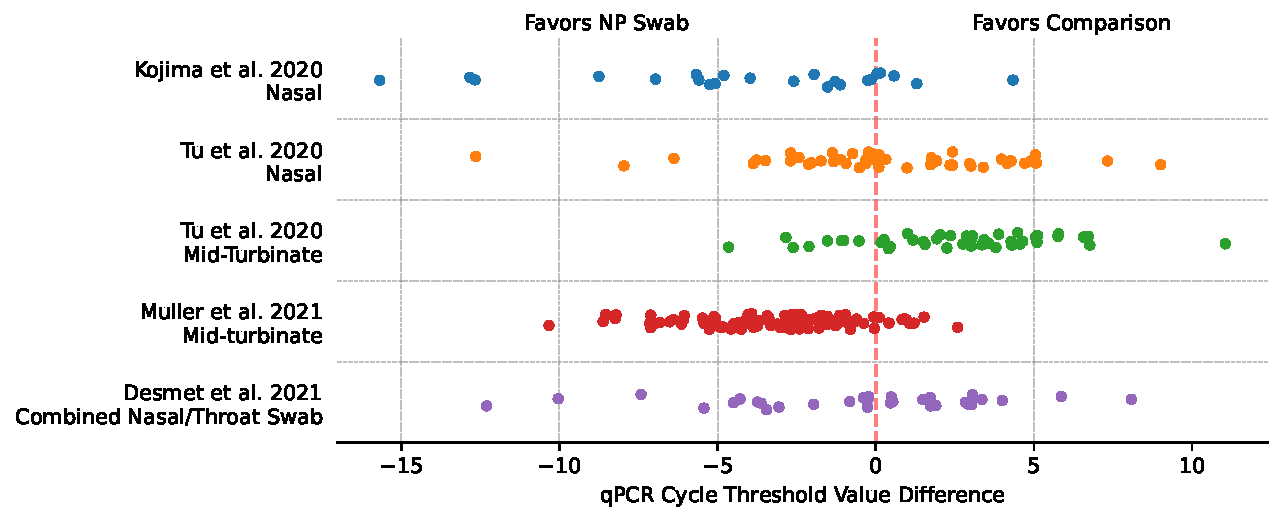
\includegraphics{index_files/figure-pdf/cell-3-output-1.pdf}

}

\caption{\textbf{Figure 1: Nasopharyngeal vs Nasal, Mid-Turbinate, and
combined Oropharyngeal/ Nasal swabs.} Data from Kojima et al.~2020, Tu
et al.~2020, Muller et al.~2021, and Desmet et al.~2021.}

\end{figure}%

Apart from self-collected mid-turbinate swabs in Tu et al.~2020, NP
swabs show equivalent performance to nasal swabs in Kojima et al.~2020,
mid-turbinate swabs in Muller et al.~2021, and combined nasal/throat
swabs in Desmet et al 2021; and equivalent performance to nasal swabs in
Tu et al.~2020. In the same study, nasal swabs prove equivalent to NP
swabs. Combined oro-pharyngeal swabs are also equivalent to NP swabs.

Studies that use NP swabs as their gold standard are useful to better
understand the performance of other swab types, but NP swabs themselves
are not practical for a large-scale pooled sampling programs: NP swabs
are notoriously uncomfortable and are commonly administered by a third
person. In contrast, nasal or oropharyngeal swabs would be more suitable
for self-sampling, which allows far higher testing throughput. Let's
thus look at studies that compare nasal and oropharyngeal swabs.

\subsubsection{Nasal Swabs}\label{nasal-swabs}

Note that the second plot shows the difference in genome copy numbers,
rather than CT values\footnote{A 1-log difference in genome copy number
  is equivalent to a 3.3 CT difference. This is because each cycle in a
  qPCR machine approxiately equates to doubling of the genome copy
  number.}.

\begin{Shaded}
\begin{Highlighting}[]
\NormalTok{df }\OperatorTok{=}\NormalTok{ pd.read\_csv(}\StringTok{"data/nasal\_ct\_differences.tsv"}\NormalTok{, sep}\OperatorTok{=}\StringTok{"}\CharTok{\textbackslash{}t}\StringTok{"}\NormalTok{, skiprows}\OperatorTok{=}\DecValTok{1}\NormalTok{)}

\NormalTok{df.columns }\OperatorTok{=}\NormalTok{ df.columns.}\BuiltInTok{str}\NormalTok{.replace(}\StringTok{", "}\NormalTok{, }\StringTok{"}\CharTok{\textbackslash{}n}\StringTok{"}\NormalTok{)}
\CommentTok{\# reshape dataframe to long format}
\NormalTok{df }\OperatorTok{=}\NormalTok{ df.melt(var\_name}\OperatorTok{=}\StringTok{"Study \& Comparison"}\NormalTok{, value\_name}\OperatorTok{=}\StringTok{"CT Difference"}\NormalTok{)}


\NormalTok{fig }\OperatorTok{=}\NormalTok{ plt.figure(figsize}\OperatorTok{=}\NormalTok{(}\DecValTok{8}\NormalTok{, }\FloatTok{1.5}\NormalTok{))}
\NormalTok{sns.stripplot(}
\NormalTok{    data}\OperatorTok{=}\NormalTok{df,}
\NormalTok{    y}\OperatorTok{=}\StringTok{"Study \& Comparison"}\NormalTok{,}
\NormalTok{    x}\OperatorTok{=}\StringTok{"CT Difference"}\NormalTok{,}
\NormalTok{    hue}\OperatorTok{=}\StringTok{"Study \& Comparison"}\NormalTok{,}
\NormalTok{    jitter}\OperatorTok{=}\VariableTok{True}\NormalTok{,}
\NormalTok{)}
\NormalTok{plt.legend([], [], frameon}\OperatorTok{=}\VariableTok{False}\NormalTok{)}
\CommentTok{\# drop y axis label}
\NormalTok{plt.ylabel(}\StringTok{""}\NormalTok{)}
\NormalTok{plt.xlabel(}\StringTok{"qPCR Cycle Threshold Value Difference"}\NormalTok{)}
\NormalTok{plt.tick\_params(axis}\OperatorTok{=}\StringTok{"y"}\NormalTok{, which}\OperatorTok{=}\StringTok{"both"}\NormalTok{, left}\OperatorTok{=}\VariableTok{False}\NormalTok{, right}\OperatorTok{=}\VariableTok{False}\NormalTok{, labelleft}\OperatorTok{=}\VariableTok{True}\NormalTok{)}

\ControlFlowTok{for}\NormalTok{ x }\KeywordTok{in} \DecValTok{5}\NormalTok{, }\DecValTok{0}\NormalTok{, }\OperatorTok{{-}}\DecValTok{5}\NormalTok{, }\OperatorTok{{-}}\DecValTok{10}\NormalTok{, }\OperatorTok{{-}}\DecValTok{15}\NormalTok{:}
    \ControlFlowTok{if}\NormalTok{ x }\OperatorTok{==} \DecValTok{0}\NormalTok{:}
\NormalTok{        plt.axvline(x}\OperatorTok{=}\NormalTok{x, color}\OperatorTok{=}\StringTok{"red"}\NormalTok{, linestyle}\OperatorTok{=}\StringTok{"{-}{-}"}\NormalTok{, alpha}\OperatorTok{=}\FloatTok{0.5}\NormalTok{)}
        \ControlFlowTok{continue}
\NormalTok{    plt.axvline(x}\OperatorTok{=}\NormalTok{x, color}\OperatorTok{=}\StringTok{"grey"}\NormalTok{, linestyle}\OperatorTok{=}\StringTok{"{-}{-}"}\NormalTok{, alpha}\OperatorTok{=}\FloatTok{0.5}\NormalTok{, linewidth}\OperatorTok{=}\FloatTok{0.5}\NormalTok{)}

\NormalTok{plt.axhline(y}\OperatorTok{=}\FloatTok{0.5}\NormalTok{, color}\OperatorTok{=}\StringTok{"grey"}\NormalTok{, linestyle}\OperatorTok{=}\StringTok{"{-}{-}"}\NormalTok{, alpha}\OperatorTok{=}\FloatTok{0.5}\NormalTok{, linewidth}\OperatorTok{=}\FloatTok{0.5}\NormalTok{)}

\NormalTok{min\_x, max\_x }\OperatorTok{=}\NormalTok{ plt.xlim()}

\NormalTok{plt.text(max\_x }\OperatorTok{/} \DecValTok{2}\NormalTok{, }\OperatorTok{{-}}\FloatTok{0.6}\NormalTok{, }\StringTok{"Favors Comparison"}\NormalTok{, fontsize}\OperatorTok{=}\DecValTok{10}\NormalTok{, color}\OperatorTok{=}\StringTok{"black"}\NormalTok{, ha}\OperatorTok{=}\StringTok{"center"}\NormalTok{)}
\NormalTok{plt.text(min\_x }\OperatorTok{/} \DecValTok{2}\NormalTok{, }\OperatorTok{{-}}\FloatTok{0.6}\NormalTok{, }\StringTok{"Favors Nasal Swab"}\NormalTok{, fontsize}\OperatorTok{=}\DecValTok{10}\NormalTok{, color}\OperatorTok{=}\StringTok{"black"}\NormalTok{, ha}\OperatorTok{=}\StringTok{"center"}\NormalTok{)}


\NormalTok{plt.gca().spines[}\StringTok{"right"}\NormalTok{].set\_visible(}\VariableTok{False}\NormalTok{)}
\NormalTok{plt.gca().spines[}\StringTok{"top"}\NormalTok{].set\_visible(}\VariableTok{False}\NormalTok{)}
\NormalTok{plt.gca().spines[}\StringTok{"left"}\NormalTok{].set\_visible(}\VariableTok{False}\NormalTok{)}

\NormalTok{plt.show()}
\end{Highlighting}
\end{Shaded}

\begin{figure}[H]

{\centering 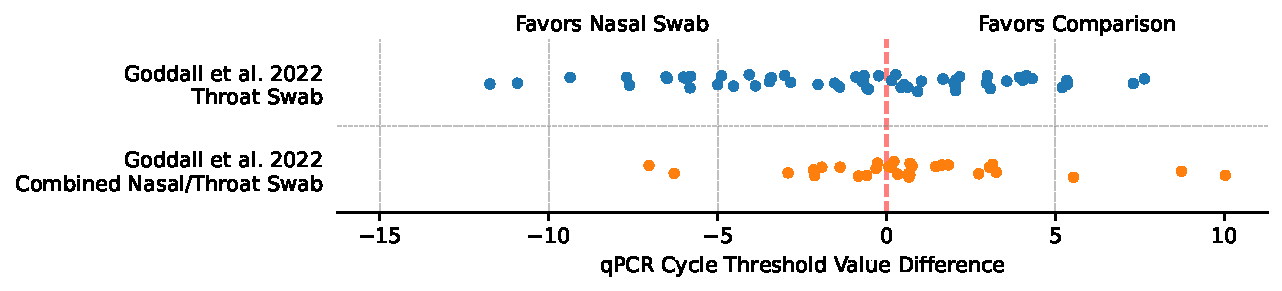
\includegraphics{index_files/figure-pdf/cell-4-output-1.pdf}

}

\caption{\textbf{Figure 2: Nasal swabs vs Oro-pharyngeal and combined
nasal/oro-pharyngeal swabs.} All data is taken from Goddall et
al.~2022.}

\end{figure}%

\begin{Shaded}
\begin{Highlighting}[]
\CommentTok{\# All CT difference data was calculated and is taken from https://docs.google.com/spreadsheets/d/1YP4mxT\_vxiFwXU5ZuBM4obq\_oscfhe05ODWwHFHEznM/}

\CommentTok{\# turn tsv into dataframe. Ignore first row. Second row is column names.}
\NormalTok{df }\OperatorTok{=}\NormalTok{ pd.read\_csv(}\StringTok{"data/leung\_genome\_copy\_differences.tsv"}\NormalTok{, sep}\OperatorTok{=}\StringTok{"}\CharTok{\textbackslash{}t}\StringTok{"}\NormalTok{, skiprows}\OperatorTok{=}\DecValTok{1}\NormalTok{)}


\NormalTok{df }\OperatorTok{=}\NormalTok{ df.melt(var\_name}\OperatorTok{=}\StringTok{"Study \& Comparison"}\NormalTok{, value\_name}\OperatorTok{=}\StringTok{"Genome Copy Number Difference"}\NormalTok{)}

\NormalTok{df[}\StringTok{"Study \& Comparison"}\NormalTok{] }\OperatorTok{=}\NormalTok{ df[}\StringTok{"Study \& Comparison"}\NormalTok{].}\BuiltInTok{str}\NormalTok{.split(}\StringTok{","}\NormalTok{).}\BuiltInTok{str}\NormalTok{[}\OperatorTok{{-}}\DecValTok{1}\NormalTok{]}
\NormalTok{fig }\OperatorTok{=}\NormalTok{ plt.figure(figsize}\OperatorTok{=}\NormalTok{(}\DecValTok{8}\NormalTok{, }\DecValTok{2}\NormalTok{))}
\NormalTok{sns.stripplot(}
\NormalTok{    data}\OperatorTok{=}\NormalTok{df,}
\NormalTok{    y}\OperatorTok{=}\StringTok{"Study \& Comparison"}\NormalTok{,}
\NormalTok{    x}\OperatorTok{=}\StringTok{"Genome Copy Number Difference"}\NormalTok{,}
\NormalTok{    hue}\OperatorTok{=}\StringTok{"Study \& Comparison"}\NormalTok{,}
\NormalTok{    jitter}\OperatorTok{=}\VariableTok{True}\NormalTok{,}
\NormalTok{)}
\NormalTok{plt.legend([], [], frameon}\OperatorTok{=}\VariableTok{False}\NormalTok{)}
\CommentTok{\# drop y axis label}
\NormalTok{plt.ylabel(}\StringTok{""}\NormalTok{)}
\NormalTok{plt.xlabel(}\StringTok{"Genome Copy Number Difference (Nasal {-} Throat Swabs), log10 scale"}\NormalTok{)}
\CommentTok{\# flip x axis}
\NormalTok{plt.gca().invert\_xaxis()}
\NormalTok{plt.tick\_params(axis}\OperatorTok{=}\StringTok{"y"}\NormalTok{, which}\OperatorTok{=}\StringTok{"both"}\NormalTok{, left}\OperatorTok{=}\VariableTok{False}\NormalTok{, right}\OperatorTok{=}\VariableTok{False}\NormalTok{, labelleft}\OperatorTok{=}\VariableTok{True}\NormalTok{)}
\ControlFlowTok{for}\NormalTok{ x }\KeywordTok{in} \OperatorTok{{-}}\DecValTok{2}\NormalTok{, }\DecValTok{0}\NormalTok{, }\DecValTok{2}\NormalTok{, }\DecValTok{4}\NormalTok{, }\DecValTok{6}\NormalTok{:}
    \ControlFlowTok{if}\NormalTok{ x }\OperatorTok{==} \DecValTok{0}\NormalTok{:}
\NormalTok{        plt.axvline(x}\OperatorTok{=}\NormalTok{x, color}\OperatorTok{=}\StringTok{"red"}\NormalTok{, linestyle}\OperatorTok{=}\StringTok{"{-}{-}"}\NormalTok{, alpha}\OperatorTok{=}\FloatTok{0.5}\NormalTok{)}
        \ControlFlowTok{continue}
\NormalTok{    plt.axvline(x}\OperatorTok{=}\NormalTok{x, color}\OperatorTok{=}\StringTok{"grey"}\NormalTok{, linestyle}\OperatorTok{=}\StringTok{"{-}{-}"}\NormalTok{, alpha}\OperatorTok{=}\FloatTok{0.5}\NormalTok{, linewidth}\OperatorTok{=}\FloatTok{0.5}\NormalTok{)}

\ControlFlowTok{for}\NormalTok{ y }\KeywordTok{in} \FloatTok{0.5}\NormalTok{, }\FloatTok{1.5}\NormalTok{:}
\NormalTok{    plt.axhline(y}\OperatorTok{=}\NormalTok{y, color}\OperatorTok{=}\StringTok{"grey"}\NormalTok{, linestyle}\OperatorTok{=}\StringTok{"{-}{-}"}\NormalTok{, alpha}\OperatorTok{=}\FloatTok{0.5}\NormalTok{, linewidth}\OperatorTok{=}\FloatTok{0.5}\NormalTok{)}

\NormalTok{min\_x, max\_x }\OperatorTok{=}\NormalTok{ plt.xlim()}

\NormalTok{plt.text(max\_x }\OperatorTok{/} \DecValTok{2}\NormalTok{, }\OperatorTok{{-}}\FloatTok{0.6}\NormalTok{, }\StringTok{"Favors Throat Swab"}\NormalTok{, fontsize}\OperatorTok{=}\DecValTok{10}\NormalTok{, color}\OperatorTok{=}\StringTok{"black"}\NormalTok{, ha}\OperatorTok{=}\StringTok{"center"}\NormalTok{)}
\NormalTok{plt.text(min\_x }\OperatorTok{/} \DecValTok{2}\NormalTok{, }\OperatorTok{{-}}\FloatTok{0.6}\NormalTok{, }\StringTok{"Favors Nasal Swab"}\NormalTok{, fontsize}\OperatorTok{=}\DecValTok{10}\NormalTok{, color}\OperatorTok{=}\StringTok{"black"}\NormalTok{, ha}\OperatorTok{=}\StringTok{"center"}\NormalTok{)}

\NormalTok{plt.gca().spines[}\StringTok{"right"}\NormalTok{].set\_visible(}\VariableTok{False}\NormalTok{)}
\NormalTok{plt.gca().spines[}\StringTok{"top"}\NormalTok{].set\_visible(}\VariableTok{False}\NormalTok{)}
\NormalTok{plt.gca().spines[}\StringTok{"left"}\NormalTok{].set\_visible(}\VariableTok{False}\NormalTok{)}

\NormalTok{plt.show()}
\end{Highlighting}
\end{Shaded}

\begin{figure}[H]

{\centering 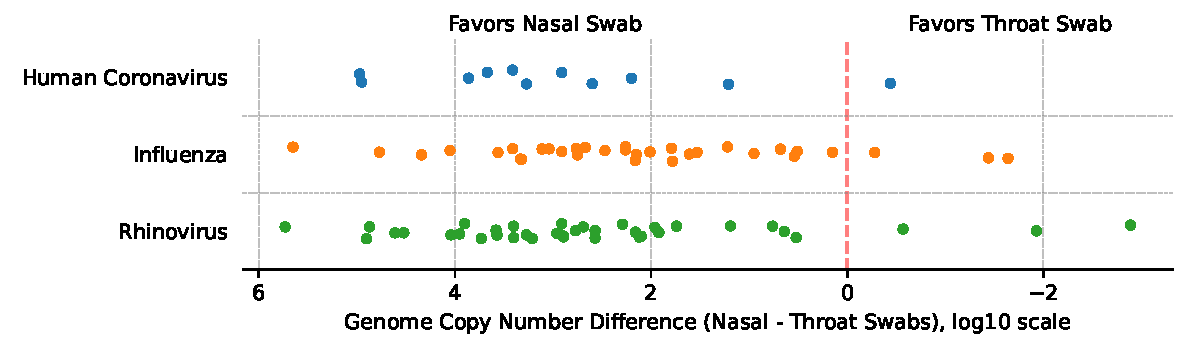
\includegraphics{index_files/figure-pdf/cell-5-output-1.pdf}

}

\caption{\textbf{Figure 3: Nasal swabs vs Oro-pharyngeal swabs.} All
data is taken from Leung et al.~2020.}

\end{figure}%

In qPCR measurements, nasal swabs contain more virus copies than throat
swabs. In (Goodall et al.~2022), nasal swabs are slightly superior to
throat swabs and combined/nasal throat swabs, and come out about even
when compared to combined nasal/OP swabs. In (Leung et al.~2020),
researchers ran multiplex-PCR on both nasal and throat swamples. qPCR
differences are plotted in Figure 3 for Human Coronavirus, Influenza,
and Rhinovirus.

\section{Virus relative abundance across different swab
types}\label{virus-relative-abundance-across-different-swab-types}

Whatever the sample type, ultimately we will want to perform metagenomic
sequencing to detect novel pathogens. As described in a
\href{https://naobservatory.org/reports/comparing-sampling-strategies-for-early-detection-of-stealth-biothreats/}{previous
report}, the value of a metagenomic sequencing sample will can be
assessed across several dimensions:

\begin{itemize}
\tightlist
\item
  What is the expected relative abundance of a human-infecting stealth
  virus?
\item
  How complex are individual sequencing samples? I.e, what is their
  species richness and evenness?
\item
  How much does the background complexity of a sample vary between
  individuals and over time?
\end{itemize}

The relative abundance of a target pathogen can be impacted by its
microbial background, because the sequencing efficiency of a taxon is
directly dependant on the sampling efficiency of the other taxa in the
sample\footnote{See
  \href{https://elifesciences.org/articles/46923}{McClaren et al.~2019}
  for further discussion.}

We identified two studies that performed paired metagenomic sequencing
and SARS-CoV-2 qPCR on swab samples Lu et al.~2021, Babiker et al.~2020.
We've reached out to the authors of two further studies that didn't have
publicly available data.

\begin{Shaded}
\begin{Highlighting}[]
\NormalTok{df\_throat }\OperatorTok{=}\NormalTok{ pd.read\_csv(}\StringTok{"data/lu\_throat\_ct\_mgs.tsv"}\NormalTok{, sep}\OperatorTok{=}\StringTok{"}\CharTok{\textbackslash{}t}\StringTok{"}\NormalTok{, skiprows}\OperatorTok{=}\DecValTok{1}\NormalTok{)}
\NormalTok{df\_throat.rename(}
\NormalTok{    columns}\OperatorTok{=}\NormalTok{\{}\StringTok{"SCV{-}2 Relative Abundance"}\NormalTok{: }\StringTok{"scv2\_ra"}\NormalTok{, }\StringTok{"Ct value"}\NormalTok{: }\StringTok{"scv2\_ct"}\NormalTok{\}, inplace}\OperatorTok{=}\VariableTok{True}
\NormalTok{)}
\NormalTok{df\_nasopharyngeal }\OperatorTok{=}\NormalTok{ pd.read\_csv(}\StringTok{"data/babiker\_np\_ct\_mgs.tsv"}\NormalTok{, sep}\OperatorTok{=}\StringTok{"}\CharTok{\textbackslash{}t}\StringTok{"}\NormalTok{, skiprows}\OperatorTok{=}\DecValTok{1}\NormalTok{)}
\NormalTok{df\_nasopharyngeal.rename(}
\NormalTok{    columns}\OperatorTok{=}\NormalTok{\{}
        \StringTok{"SARS{-}CoV{-}2 RT{-}PCR Ct"}\NormalTok{: }\StringTok{"scv2\_ct"}\NormalTok{,}
        \StringTok{"SARS{-}CoV{-}2 RA"}\NormalTok{: }\StringTok{"scv2\_ra"}\NormalTok{,}
        \StringTok{"Inpatient/ED vs. Outpatient"}\NormalTok{: }\StringTok{"patient\_status"}\NormalTok{,}
\NormalTok{    \},}
\NormalTok{    inplace}\OperatorTok{=}\VariableTok{True}\NormalTok{,}
\NormalTok{)}
\NormalTok{df\_nasopharyngeal[}\StringTok{"scv2\_ct"}\NormalTok{] }\OperatorTok{=}\NormalTok{ (}
\NormalTok{    df\_nasopharyngeal[}\StringTok{"scv2\_ct"}\NormalTok{].replace(}\StringTok{","}\NormalTok{, }\StringTok{"."}\NormalTok{, regex}\OperatorTok{=}\VariableTok{True}\NormalTok{).astype(}\BuiltInTok{float}\NormalTok{)}
\NormalTok{)}

\NormalTok{fig, axs }\OperatorTok{=}\NormalTok{ plt.subplots(}\DecValTok{2}\NormalTok{, }\DecValTok{1}\NormalTok{, figsize}\OperatorTok{=}\NormalTok{(}\DecValTok{9}\NormalTok{, }\DecValTok{6}\NormalTok{))}
\ControlFlowTok{for}\NormalTok{ i, (ax, df) }\KeywordTok{in} \BuiltInTok{enumerate}\NormalTok{(}\BuiltInTok{zip}\NormalTok{(axs, [df\_throat, df\_nasopharyngeal])):}
\NormalTok{    x\_lim }\OperatorTok{=} \FloatTok{12.5}\NormalTok{, }\FloatTok{37.5}
    \ControlFlowTok{if}\NormalTok{ i }\OperatorTok{==} \DecValTok{1}\NormalTok{:}
        \CommentTok{\# set dot colors}
\NormalTok{        sns\_default\_colors }\OperatorTok{=}\NormalTok{ sns.color\_palette(}\StringTok{"tab10"}\NormalTok{)}
\NormalTok{        sns.scatterplot(}
\NormalTok{            ax}\OperatorTok{=}\NormalTok{ax,}
\NormalTok{            data}\OperatorTok{=}\NormalTok{df,}
\NormalTok{            x}\OperatorTok{=}\StringTok{"scv2\_ct"}\NormalTok{,}
\NormalTok{            y}\OperatorTok{=}\StringTok{"scv2\_ra"}\NormalTok{,}
\NormalTok{            hue}\OperatorTok{=}\StringTok{"patient\_status"}\NormalTok{,}
\NormalTok{            style}\OperatorTok{=}\StringTok{"patient\_status"}\NormalTok{,}
\NormalTok{            s}\OperatorTok{=}\DecValTok{100}\NormalTok{,}
\NormalTok{            palette}\OperatorTok{=}\NormalTok{sns\_default\_colors[}\DecValTok{2}\NormalTok{:}\DecValTok{4}\NormalTok{],}
\NormalTok{        )}
        \CommentTok{\# set coordinates for legend}
\NormalTok{        coordinates }\OperatorTok{=}\NormalTok{ (}\FloatTok{0.6}\NormalTok{, }\OperatorTok{{-}}\FloatTok{0.2}\NormalTok{)}
\NormalTok{        ax.legend(title}\OperatorTok{=}\StringTok{""}\NormalTok{, loc}\OperatorTok{=}\StringTok{"upper left"}\NormalTok{)  }\CommentTok{\# bbox\_to\_anchor=coordinates)}
\NormalTok{        ax.set\_xlabel(}\StringTok{"SARS{-}CoV{-}2 qPCR CT Value"}\NormalTok{)}
\NormalTok{        ax.set\_xlim(x\_lim)}
    \ControlFlowTok{else}\NormalTok{:}
\NormalTok{        sns.scatterplot(ax}\OperatorTok{=}\NormalTok{ax, data}\OperatorTok{=}\NormalTok{df, x}\OperatorTok{=}\StringTok{"scv2\_ct"}\NormalTok{, y}\OperatorTok{=}\StringTok{"scv2\_ra"}\NormalTok{, s}\OperatorTok{=}\DecValTok{100}\NormalTok{)}
\NormalTok{        ax.set\_xlabel(}\StringTok{""}\NormalTok{)}
\NormalTok{        ax.set\_xlim(x\_lim)}
\NormalTok{    ax.set\_yscale(}\StringTok{"log"}\NormalTok{)}
\NormalTok{    ax.invert\_xaxis()}
\NormalTok{    ax.spines[}\StringTok{"right"}\NormalTok{].set\_visible(}\VariableTok{False}\NormalTok{)}
\NormalTok{    ax.spines[}\StringTok{"top"}\NormalTok{].set\_visible(}\VariableTok{False}\NormalTok{)}
\NormalTok{    ax.tick\_params(axis}\OperatorTok{=}\StringTok{"y"}\NormalTok{, which}\OperatorTok{=}\StringTok{"both"}\NormalTok{, left}\OperatorTok{=}\VariableTok{False}\NormalTok{, right}\OperatorTok{=}\VariableTok{False}\NormalTok{, labelleft}\OperatorTok{=}\VariableTok{True}\NormalTok{)}
\NormalTok{    ax.set\_ylabel(}\StringTok{"Relative Abundance"}\NormalTok{)}
    \ControlFlowTok{for}\NormalTok{ x }\KeywordTok{in}\NormalTok{ np.arange(}\DecValTok{15}\NormalTok{, }\FloatTok{37.5}\NormalTok{, }\FloatTok{2.5}\NormalTok{):}
\NormalTok{        ax.axvline(x}\OperatorTok{=}\NormalTok{x, color}\OperatorTok{=}\StringTok{"grey"}\NormalTok{, linestyle}\OperatorTok{=}\StringTok{"{-}{-}"}\NormalTok{, alpha}\OperatorTok{=}\FloatTok{0.5}\NormalTok{, linewidth}\OperatorTok{=}\FloatTok{0.5}\NormalTok{)}
    \ControlFlowTok{for}\NormalTok{ y }\KeywordTok{in} \BuiltInTok{range}\NormalTok{(}\OperatorTok{{-}}\DecValTok{7}\NormalTok{, }\DecValTok{1}\NormalTok{, }\DecValTok{1}\NormalTok{):}
\NormalTok{        log\_y }\OperatorTok{=} \DecValTok{10}\OperatorTok{**}\NormalTok{y}
\NormalTok{        ax.axhline(y}\OperatorTok{=}\NormalTok{log\_y, color}\OperatorTok{=}\StringTok{"grey"}\NormalTok{, linestyle}\OperatorTok{=}\StringTok{"{-}{-}"}\NormalTok{, alpha}\OperatorTok{=}\FloatTok{0.5}\NormalTok{, linewidth}\OperatorTok{=}\FloatTok{0.5}\NormalTok{)}
\end{Highlighting}
\end{Shaded}

\begin{figure}[H]

{\centering 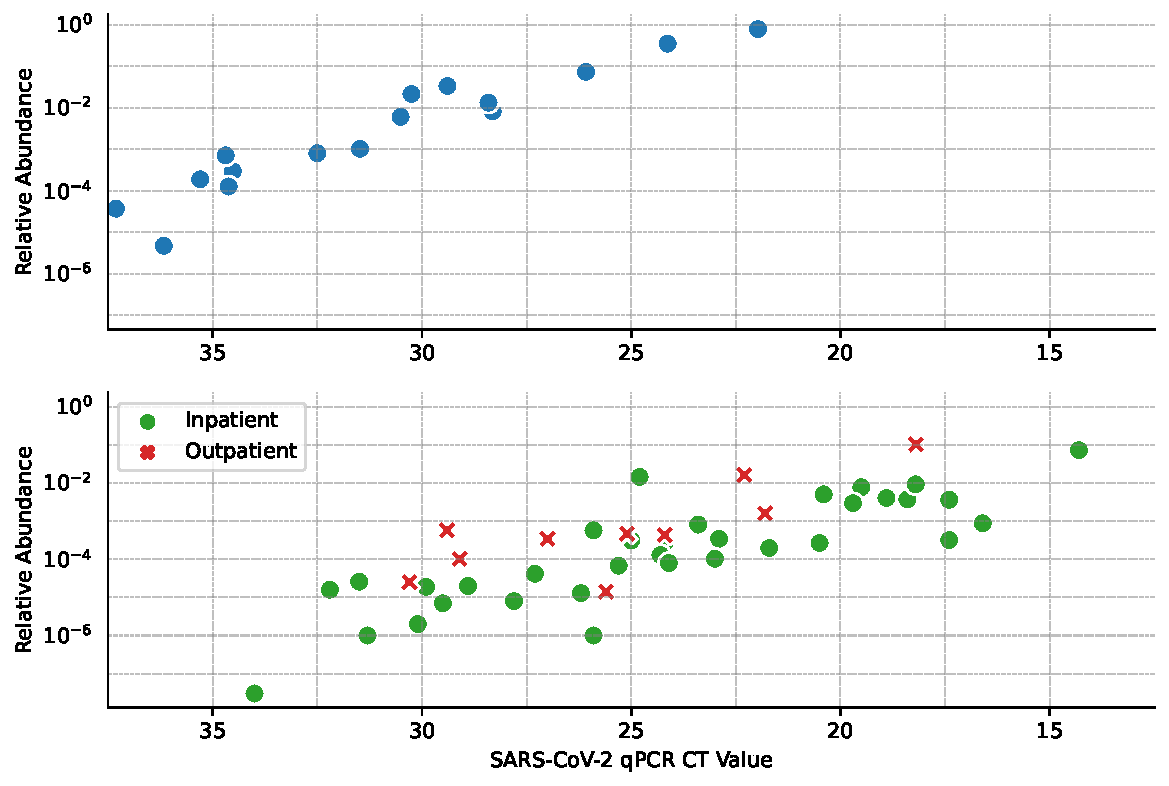
\includegraphics{index_files/figure-pdf/cell-6-output-1.pdf}

}

\caption{\textbf{Figure 4: SARS-CoV-2 qPCR CT vs SARS-CoV-2 RA.} Top
Figure: Throat Swabs. Data from Lu et al.~2021. Bottom Figure:
Nasopharyngeal Swabs. Data from Babiker et al.~2020.}

\end{figure}%

Some observations:

\begin{itemize}
\tightlist
\item
  Though comparing qPCR values between studies is tricky, we do see the
  expected difference in CT values, where nasopharyngeal swabs have
  lower CT values.
\item
  For the same CT value, Lu et al.~2021 returns higher relative
  abundance.
\item
  Outpatients in Lu et al.~have slightly higher relative abundances for
  the same CT value.
\end{itemize}

\section{Simulating detection
capability}\label{simulating-detection-capability}

We can use the above data to replicate research by Jeff Kaufman. Let's
say we get a random set of swabs from a population which contains 1\%
sick people. On average 1\% of all swabs will return positive, and the
relative abundance in that positive sample is picked randomly among the
relative abundances given in Lu et al.~2021 and Babiker et al.~2020,
respectively.

Based on this, the median RA(1\%) in a pooled sample with 200 swabs is
\textasciitilde{} 10\^{}-4.8 Lu et al.~2021 (throat swabs) and
10\^{}-5.9 in Babiker et al.~2020 (NP swabs)

\begin{Shaded}
\begin{Highlighting}[]
\KeywordTok{def}\NormalTok{ simulate\_detection(positive\_ras):}
\NormalTok{    FRAC\_SICK }\OperatorTok{=} \FloatTok{0.01}
\NormalTok{    SIMULATIONS }\OperatorTok{=} \DecValTok{10000}

    \KeywordTok{def}\NormalTok{ probabilistic\_round(x):}
        \ControlFlowTok{return} \BuiltInTok{int}\NormalTok{(math.floor(x }\OperatorTok{+}\NormalTok{ random.random()))}

    \KeywordTok{def}\NormalTok{ simulate\_once(n\_swabs):}
\NormalTok{        n\_sick }\OperatorTok{=}\NormalTok{ probabilistic\_round(FRAC\_SICK }\OperatorTok{*}\NormalTok{ n\_swabs)}
        \ControlFlowTok{if} \KeywordTok{not}\NormalTok{ n\_sick:}
            \ControlFlowTok{return} \DecValTok{0}
\NormalTok{        ra }\OperatorTok{=} \DecValTok{0}
        \ControlFlowTok{for}\NormalTok{ \_ }\KeywordTok{in} \BuiltInTok{range}\NormalTok{(n\_sick):}
\NormalTok{            ra }\OperatorTok{=}\NormalTok{ random.choice(positive\_ras)}
        \ControlFlowTok{return}\NormalTok{ ra }\OperatorTok{/}\NormalTok{ n\_swabs}

    \KeywordTok{def}\NormalTok{ simulate\_many(n\_simulations, n\_swabs):}
\NormalTok{        RAs }\OperatorTok{=}\NormalTok{ []}
        \ControlFlowTok{for}\NormalTok{ \_ }\KeywordTok{in} \BuiltInTok{range}\NormalTok{(n\_simulations):}
\NormalTok{            RAs.append(simulate\_once(n\_swabs))}
\NormalTok{        RAs.sort()}

        \ControlFlowTok{return}\NormalTok{ [}
\NormalTok{            RAs[probabilistic\_round(}\BuiltInTok{len}\NormalTok{(RAs) }\OperatorTok{*}\NormalTok{ percentile }\OperatorTok{/} \DecValTok{100}\NormalTok{)]}
            \ControlFlowTok{for}\NormalTok{ percentile }\KeywordTok{in} \BuiltInTok{range}\NormalTok{(}\DecValTok{100}\NormalTok{)}
\NormalTok{        ]}

\NormalTok{    data }\OperatorTok{=}\NormalTok{ defaultdict(}\BuiltInTok{list}\NormalTok{)}
\NormalTok{    n\_swab\_range }\OperatorTok{=}\NormalTok{ [}\DecValTok{50}\NormalTok{, }\DecValTok{100}\NormalTok{, }\DecValTok{200}\NormalTok{, }\DecValTok{400}\NormalTok{, }\DecValTok{800}\NormalTok{]}
    \ControlFlowTok{for}\NormalTok{ n\_swabs }\KeywordTok{in}\NormalTok{ n\_swab\_range:}
        \ControlFlowTok{for}\NormalTok{ percentile, ra }\KeywordTok{in} \BuiltInTok{enumerate}\NormalTok{(simulate\_many(SIMULATIONS, n\_swabs)):}
\NormalTok{            data[percentile].append(ra)}
\NormalTok{    df }\OperatorTok{=}\NormalTok{ pd.DataFrame(data).T}
\NormalTok{    df.columns }\OperatorTok{=}\NormalTok{ n\_swab\_range}

    \ControlFlowTok{return}\NormalTok{ df}


\NormalTok{df\_throat }\OperatorTok{=}\NormalTok{ pd.read\_csv(}\StringTok{"data/lu\_throat\_ct\_mgs.tsv"}\NormalTok{, sep}\OperatorTok{=}\StringTok{"}\CharTok{\textbackslash{}t}\StringTok{"}\NormalTok{, skiprows}\OperatorTok{=}\DecValTok{1}\NormalTok{)}
\NormalTok{df\_throat.rename(}
\NormalTok{    columns}\OperatorTok{=}\NormalTok{\{}\StringTok{"SCV{-}2 Relative Abundance"}\NormalTok{: }\StringTok{"scv2\_ra"}\NormalTok{, }\StringTok{"Ct value"}\NormalTok{: }\StringTok{"scv2\_ct"}\NormalTok{\}, inplace}\OperatorTok{=}\VariableTok{True}
\NormalTok{)}

\NormalTok{df\_nasopharyngeal }\OperatorTok{=}\NormalTok{ pd.read\_csv(}\StringTok{"data/babiker\_np\_ct\_mgs.tsv"}\NormalTok{, sep}\OperatorTok{=}\StringTok{"}\CharTok{\textbackslash{}t}\StringTok{"}\NormalTok{, skiprows}\OperatorTok{=}\DecValTok{1}\NormalTok{)}
\NormalTok{df\_nasopharyngeal.rename(}
\NormalTok{    columns}\OperatorTok{=}\NormalTok{\{}
        \StringTok{"SARS{-}CoV{-}2 RT{-}PCR Ct"}\NormalTok{: }\StringTok{"scv2\_ct"}\NormalTok{,}
        \StringTok{"SARS{-}CoV{-}2 RA"}\NormalTok{: }\StringTok{"scv2\_ra"}\NormalTok{,}
        \StringTok{"Inpatient/ED vs. Outpatient"}\NormalTok{: }\StringTok{"patient\_status"}\NormalTok{,}
\NormalTok{    \},}
\NormalTok{    inplace}\OperatorTok{=}\VariableTok{True}\NormalTok{,}
\NormalTok{)}
\NormalTok{df\_nasopharyngeal[}\StringTok{"scv2\_ct"}\NormalTok{] }\OperatorTok{=}\NormalTok{ (}
\NormalTok{    df\_throat[}\StringTok{"scv2\_ct"}\NormalTok{].replace(}\StringTok{","}\NormalTok{, }\StringTok{"."}\NormalTok{, regex}\OperatorTok{=}\VariableTok{True}\NormalTok{).astype(}\BuiltInTok{float}\NormalTok{)}
\NormalTok{)}

\NormalTok{df\_throat\_ras }\OperatorTok{=}\NormalTok{ df\_throat[}\StringTok{"scv2\_ra"}\NormalTok{].dropna().tolist()}
\NormalTok{df\_nasopharyngeal\_ras }\OperatorTok{=}\NormalTok{ df\_nasopharyngeal[}\StringTok{"scv2\_ra"}\NormalTok{].dropna().tolist()}
\NormalTok{fig, axs }\OperatorTok{=}\NormalTok{ plt.subplots(}\DecValTok{1}\NormalTok{, }\DecValTok{2}\NormalTok{, figsize}\OperatorTok{=}\NormalTok{(}\DecValTok{9}\NormalTok{, }\DecValTok{5}\NormalTok{), sharey}\OperatorTok{=}\VariableTok{True}\NormalTok{)}
\NormalTok{n\_swab\_range }\OperatorTok{=}\NormalTok{ [}\DecValTok{50}\NormalTok{, }\DecValTok{100}\NormalTok{, }\DecValTok{200}\NormalTok{, }\DecValTok{400}\NormalTok{, }\DecValTok{800}\NormalTok{]}
\ControlFlowTok{for}\NormalTok{ i, positive\_ras }\KeywordTok{in} \BuiltInTok{enumerate}\NormalTok{([df\_throat\_ras, df\_nasopharyngeal\_ras]):}
\NormalTok{    df }\OperatorTok{=}\NormalTok{ simulate\_detection(positive\_ras)}
    \ControlFlowTok{for}\NormalTok{ n\_swabs }\KeywordTok{in}\NormalTok{ n\_swab\_range:}
\NormalTok{        axs[i].plot(df.index, df[n\_swabs], label}\OperatorTok{=}\SpecialStringTok{f"}\SpecialCharTok{\{}\NormalTok{n\_swabs}\SpecialCharTok{\}}\SpecialStringTok{ swabs"}\NormalTok{)}
\NormalTok{    axs[i].set\_xlabel(}\StringTok{"Percentile"}\NormalTok{)}
\NormalTok{    axs[i].set\_ylabel(}\StringTok{"RA"}\NormalTok{)}
\NormalTok{    axs[i].set\_yscale(}\StringTok{"log"}\NormalTok{)}
    \CommentTok{\# turn on y tick labels for both plots}
\NormalTok{    axs[i].yaxis.set\_tick\_params(labelleft}\OperatorTok{=}\VariableTok{True}\NormalTok{)}
    \ControlFlowTok{for}\NormalTok{ x }\KeywordTok{in} \BuiltInTok{range}\NormalTok{(}\DecValTok{0}\NormalTok{, }\DecValTok{100}\NormalTok{, }\DecValTok{20}\NormalTok{):}
\NormalTok{        axs[i].axvline(x}\OperatorTok{=}\NormalTok{x, color}\OperatorTok{=}\StringTok{"black"}\NormalTok{, linestyle}\OperatorTok{=}\StringTok{"{-}{-}"}\NormalTok{, linewidth}\OperatorTok{=}\FloatTok{0.5}\NormalTok{, alpha}\OperatorTok{=}\FloatTok{0.5}\NormalTok{)}

    \ControlFlowTok{for}\NormalTok{ y }\KeywordTok{in} \BuiltInTok{range}\NormalTok{(}\OperatorTok{{-}}\DecValTok{1}\NormalTok{, }\OperatorTok{{-}}\DecValTok{10}\NormalTok{, }\OperatorTok{{-}}\DecValTok{1}\NormalTok{):}
\NormalTok{        log\_y }\OperatorTok{=} \DecValTok{10}\OperatorTok{**}\NormalTok{y}
\NormalTok{        axs[i].axhline(y}\OperatorTok{=}\NormalTok{log\_y, color}\OperatorTok{=}\StringTok{"black"}\NormalTok{, linestyle}\OperatorTok{=}\StringTok{"{-}{-}"}\NormalTok{, linewidth}\OperatorTok{=}\FloatTok{0.5}\NormalTok{, alpha}\OperatorTok{=}\FloatTok{0.5}\NormalTok{)}
    \ControlFlowTok{if}\NormalTok{ i }\OperatorTok{==} \DecValTok{0}\NormalTok{:}
\NormalTok{        axs[i].set\_title(}\StringTok{"Throat"}\NormalTok{)}
    \ControlFlowTok{else}\NormalTok{:}
\NormalTok{        axs[i].set\_title(}\StringTok{"Nasopharyngeal"}\NormalTok{)}

\NormalTok{    axs[i].spines[}\StringTok{"right"}\NormalTok{].set\_visible(}\VariableTok{False}\NormalTok{)}
\NormalTok{    axs[i].spines[}\StringTok{"top"}\NormalTok{].set\_visible(}\VariableTok{False}\NormalTok{)}
\NormalTok{    ax.tick\_params(axis}\OperatorTok{=}\StringTok{"x"}\NormalTok{, which}\OperatorTok{=}\StringTok{"both"}\NormalTok{, bottom}\OperatorTok{=}\VariableTok{False}\NormalTok{, top}\OperatorTok{=}\VariableTok{False}\NormalTok{, labelbottom}\OperatorTok{=}\VariableTok{True}\NormalTok{)}
    \ControlFlowTok{if}\NormalTok{ i }\OperatorTok{==} \DecValTok{1}\NormalTok{:}
\NormalTok{        axs[i].legend()}
\end{Highlighting}
\end{Shaded}

\begin{figure}[H]

{\centering 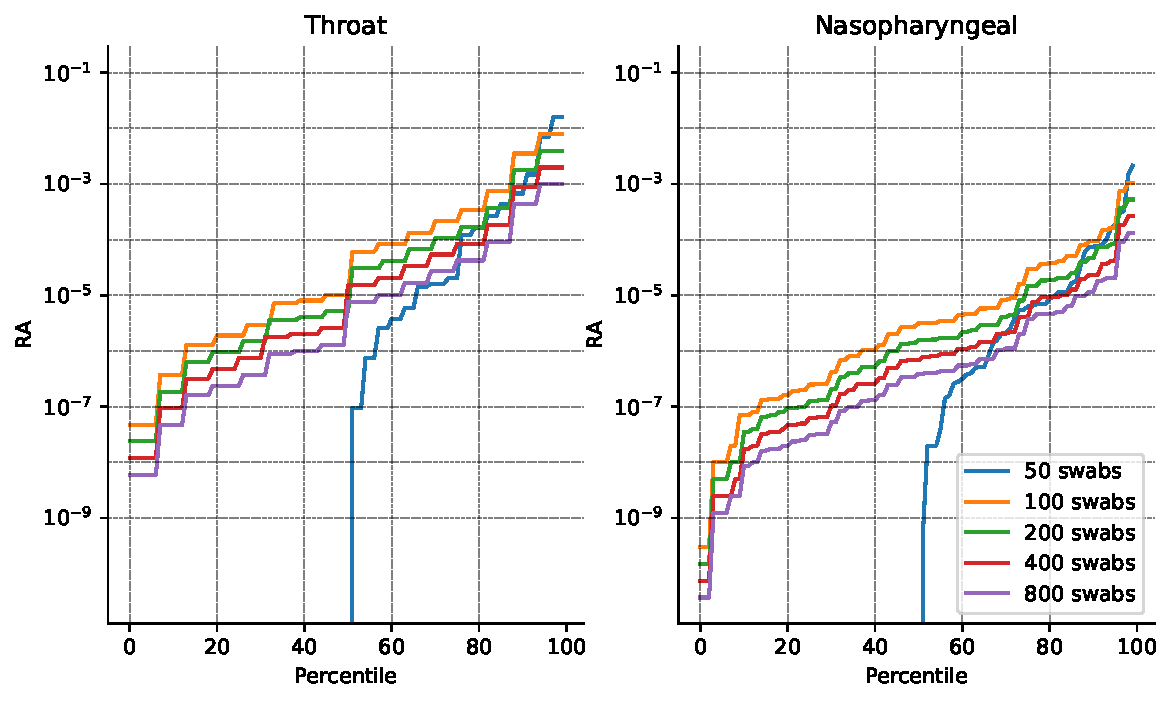
\includegraphics{index_files/figure-pdf/cell-7-output-1.pdf}

}

\caption{\textbf{Figure 5: Simulated detection capability of pooled swab
sampling.} Left Figure: Throat Swabs. Data from Lu et al.~2021. Right
Figure: Nasopharyngeal Swabs. Data from Babiker et al.~2020.}

\end{figure}%

\subsection{Next steps}\label{next-steps}

\begin{itemize}
\tightlist
\item
  Pull in additional qPCR studies.
\item
  Read into research on comparing CT values across studies and search
  for standard curves in existing papers.
\item
  Lay out what you would do if you had standard curves available.
\end{itemize}

Create a figure for the remaining viruses not covered in Figure 3.



\end{document}
